\documentclass[../proyecto.tex]{book}

\begin{document}

\chapter{Introducción}

El autómata celular fue inventado por von Neumann y Ulam en 1950 para estudiar el problema de construir máquinas artificiales que se reproduzcan a sí mismas \cite{neummanUlam}. Con el fin de imitar el comportamiento de los seres vivos, el diseño de dichas máquinas incluye el espacio en el que se desarrollan, representado por una malla rectangular en la que en los nodos se sitúan células y éstas evolucionan simultáneamente de acuerdo a un conjunto de reglas simples que dirigen la \textit{física} de su pequeño universo abstracto. 

El juego de vida es un autómata celular propuesto por Conway en 1970 y popularizado por Gardner en el mismo año \cite{primerap}. Consiste en la evolución de una disposición inicial de células en dos estados mutuamente excluyentes, vida (1) o muerte (0), en una malla rectangular infinita. Dicha evolución viene regida por un conjunto de reglas que se aplican simultáneamente a todas las células en cada iteración. Las reglas son las siguientes: dada una célula viva, ésta continua viviendo solo si en su vecindario hay dos o tres células, en otro caso muere; dada una célula muerta, ésta renace si tiene exactamente tres células en su vecindario. Usualmente se consideran como pertenecientes al vecindario las células adyacentes en las direcciones horizontal, vertical y diagonales.

Uno de los motivos que atrajo la atención de científicos de diversos campos hacia el juego de vida fue observar cómo patrones complejos surgen de la aplicación de un conjunto muy simple y reducido de reglas. De esta manera comenzaron a analizarse configuraciones iniciales que daban lugar a comportamientos interesantes, tales como \textit{glider} \autoref{fig:1-1} que se desplaza sobre la malla, \textit{blinker} \autoref{fig:1-3} que retorna a su configuración inicial tras un número finito de iteraciones o \textit{block} \autoref{fig:1-2} que no ve alterado su forma en cada iteración.

\begin{figure}[H]
	\centering
	\begin{subfigure}[b]{0.3\linewidth} 
        \centering
        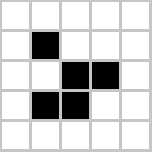
\includegraphics[height=.6\linewidth]{./images/glider.png}
        \caption{}
        \label{fig:1-1}
    \end{subfigure}
    \quad
	\begin{subfigure}[b]{0.3\linewidth} 
        \centering
        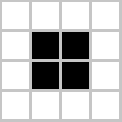
\includegraphics[height=.55\linewidth]{./images/block.png}
        \caption{}
        \label{fig:1-2}
    \end{subfigure}
	\\    
    \begin{subfigure}[b]{0.3\linewidth} 
        \centering
        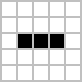
\includegraphics[height=0.45\linewidth]{./images/blinker.png}
        \caption{}
        \label{fig:1-3}
    \end{subfigure}
	\caption{Configuraciones iniciales del juego de vida.}
	\label{fig:congIniciales}
\end{figure} 


La elección de las reglas de evolución parecería \textit{a priori} aleatoria, sin embargo, Conway las escogió de acorde a las siguientes pautas \cite{libroGardner}:
\begin{itemize}
	\item No debe existir una disposición inicial de células para la cual haya una prueba simple de que la población crezca sin límite.
	\item Debe haber disposiciones iniciales de células que aparentemente crezcan sin límite. 
	\item Debe haber disposiciones iniciales de células simples que crezcan y cambien durante un periodo relativamente largo, llegando a tres posibles finales: desaparecer completamente ya sea debido a superpoblación o a dispersión, estabilizarse en una configuración que se mantenga constante o entrar en un ciclo sin fin de oscilación.
\end{itemize}

Al intentar realizar simulaciones de juegos de vida, los ordenadores se erigieron como la herramienta principal para llevarlas a cabo, siendo necesario afrontar el problema de representar una malla rectangular infinita en un ordenador con memoria finita. Una inteligente solución es alterar las características topológicas de la malla rectangular, identificando los bordes opuestos para obtener superficies topológicamente equivalentes a las de una botella de Klein, una esfera o un toro. En particular, esta última resultó atraer gran interés, pues se encontraron evidencias de que reduce los efectos asociados a la finitud de la malla \cite{finitudMalla, finitudMalla2}. Cabe también descatar el estudio de la alteración de las cualidades geométricas de la malla, tales como el uso de figuras geométricas diferentes al cuadrado (triángulo y hexágono)\cite{triangular}, teselaciones de Penrose \cite{penrose} o el empleo del espacio geométrico hiperbólico \cite{hiperbolico}. Finalmente, existen implementaciones en las cuales no se almacena la malla en la memoria, si no que se almacena la posición de cada célula respecto a un origen de coordenadas, simulando más eficazmente una malla  rectangular infinita \cite{boardless}.

El juego de vida de Conway también muestra interesantes características en el campo de la teoría de la computación, pertenece a la clase IV de Wolfram, esto es, su evolución lleva a estructuras aisladas que muestran un comportamiento complejo \cite{ccuatro, ccuatro2}. Se ha demostrado que tiene la capacidad de cómputo de una máquina de Turing universal. Por tanto existe una disposición inicial de células que simula una máquina de Turing, la cual fue extendida a una máquina universal de Turing \cite{turingUniversal,turing}. Como muestra de dicha capacidad de computación, en un esfuerzo colectivo se ha implementado sobre éste un ordenador con su propio lenguaje de ensamblador y de alto nivel, y se ha programado el conocido juego Tetris \cite{tetris, logical}.

Si los autómatas celulares son un modelo que representa organismos vivos se podría pensar que la hipótesis de actualización simultánea es cuestionable ya que en la naturaleza no se propaga la información de manera instantánea y mucho menos de manera perfecta. Es ese aspecto, que está ligado a la robustez del modelo frente a perturbaciones en su evolución, el que pretendemos analizar en este trabajo. Un modelo será robusto si pequeños cambios en su evolución se traducen en pequeñas perturbaciones del comportamiento global del sistema, mientras que si esta pequeña modificación produce un cambio cualitativo en la dinámica, el sistema será poco robusto o, simplemente, se tratará de un sistema muy sensible a las variaciones que puedan ocurrir en sus elementos. En algunos contextos, los cambios cualitativos a los que nos referimos aquí se conocen como transición de fase. En la bibliografía la introducción de estas perturbaciones se lleva a cabo a través de la asincronicidad en la aplicación reglas de evolución \cite{asyncIntro}. Se pueden considerar las siguientes opciones:
\begin{itemize}
	\item \textbf{Evolución totalmente asíncrona}. En cada iteración, las reglas de evolución se aplican solamente a un individuo escogido del conjunto de células, el criterio de elección puede ser o no ser completamente aleatorio.
	\item \textbf{Evolución $\alpha$-asíncrona}. En cada iteración, cada célula tiene probabilidad $\alpha$ de que se le apliquen las reglas de evolución y probabilidad $1-\alpha$ de mantener su estado.
\end{itemize}

Estos esquemas de evolución también se conocen como \textbf{evolución guiada por pasos} y \textbf{evolución guiada por tiempo}, respectivamente \cite{aka}. Los primeros en estudiar los efectos de la evolución asíncrona frente a la evolución síncrona en el juego de vida fueron Blok y Bergersen \cite{syncVSasync}: aplicando un esquema de evolución $\alpha$-asíncrona demostraron la existencia de una transición de fase de un comportamiento \"estático\", donde el sistema termina alcanzando alguna situación completamente estable, a un comportamiento \textit{vívido} y, por tanto, inestable. Posteriormente se estudió cómo afectaban las variaciones en la topología de la malla a la transición de fase, concluyendo que su aparición depende fuertemente de la regularidad de la malla rectángular \cite{mallaIrregular}. Debido a que no existe una definición globalmente aceptada de autómata celular que agrupe los dos esquemas de actualización asíncrona anteriores, proponemos la definición de autómata celular m-asíncrono dada en \cite{oraculo}. 

Hasta donde podemos saber solo se ha estudiado el comportamiento en situaciones de $\alpha$-asincronicidad de configuraciones iniciales aleatorias, también conocidas como \textit{sopas}, con una densidad prefijada, obteniendo resultados que se comparan con las características conocidas del juego de vida síncrono. En este trabajo queremos caracterizar la manera en la que configuraciones iniciales bien conocidas y estudiadas, como las que se muestran en la figura \ref{fig:congIniciales}, alteran su comportamiento en situaciones de $\alpha$-asincronicidad. Utilizaremos las técnicas Monte Calo para medir diferentes variables tales como el crecimiento de la población, el número de cúmulos de células y la actividad de nacimiento y muerte de células.

El capítulo 2 está dedicado a una descripción de los aspectos esenciales de nuestro trabajo. A continuación el capítulo 3 se proporciona una visión más formal de los conceptos expuestos en el capítulo anterior. En el capítulo 4 se documentan los resultados obtenidos y se discuten los aspectos más relevantes de los mismos. Por último en el capítulo 5 se establecen las conclusiones de nuestro trabajo. 

\end{document}

% !TeX root = ../proyecto.tex
